% Nivio: 29/jan/06
% Time-stamp: <Monday 30 Jan 2006 12:13:14pm EST yoshi@flare>
\subsection{Performance of the new algorithm}
\label{sec:performance}
%As we have done for the internal memory based algorithm, 

The runtime of our algorithm is also a random variable, but now it follows a
(highly concentrated) normal distribution, as we discuss at the end of this
section.  Again, we are interested in verifying the linearity claim made in
Section~\ref{sec:linearcomplexity}.  Therefore, we ran the algorithm for
several numbers $n$ of keys in $S$.

The values chosen for $n$ were $1, 2, 4, 8, 16, 32, 64, 128, 512$ and $1000$
million. 
%Just the small vector {\it size} must be kept in main memory,
%as we saw in Section~\ref{sec:memconstruction}.
We limited the main memory in 500 megabytes for the experiments.
The size $\mu$ of the a priori reserved internal memory area 
was set to 250 megabytes, the parameter $b$ was set to $175$ and
the building block algorithm parameter $c$ was again set to $1$.
In Section~\ref{sec:contr-disk-access} we show how $\mu$
affects the runtime of the algorithm. The other two parameters
have insignificant influence on the runtime.  

We again use a statistical method for determining a suitable sample size
%~\cite[Chapter 13]{j91}
to estimate the number of trials to be run for each value of $n$.  We got that
just one trial for each $n$ would be enough with a confidence level of $95\%$.
However, we made 10 trials.  This number of trials seems rather small, but, as
shown below, the behavior of our algorithm is very stable and its runtime is
almost deterministic (i.e., the standard deviation is very small).
 
Table~\ref{tab:mediasbrz} presents the runtime average for each $n$,
the respective standard deviations, and 
the respective confidence intervals given by 
the average time $\pm$ the distance from average time
considering a confidence level of $95\%$.
Observing the runtime averages we noticed that 
the algorithm runs in expected linear time, 
as shown in~Section~\ref{sec:linearcomplexity}.  Better still,
it is only approximately $60\%$  slower than our internal memory based algorithm.
To get that value we used the linear regression model obtained for the runtime of
the internal memory based algorithm to estimate how much time it would require
for constructing a MPHF for a set of 1 billion keys. 
We got 2.3 hours for the internal memory based algorithm  and we measured  
3.67 hours on average for our algorithm. 
Increasing the size of the internal memory area 
from 250 to 600 megabytes (see Section~\ref{sec:contr-disk-access}),
we have brought the time to 3.09 hours. In this case, our algorithm is 
just $34\%$  slower in this setup.

\enlargethispage{2\baselineskip}
\begin{table*}[htb]
\vspace{-1mm}
\begin{center}
{\scriptsize
\begin{tabular}{|l|c|c|c|c|c|}
\hline
$n$ (millions)   & 1                  & 2                  & 4                  & 8                   & 16             \\
\hline % Part.      16 \%                 16 \%                 16 \%                18 \%                 20\%           
Average time (s) & $6.9 \pm 0.3$  & $13.8 \pm 0.2$ & $31.9 \pm 0.7$ & $69.9 \pm 1.1$  & $140.6 \pm 2.5$  \\
SD               & $0.4$            & $0.2$            & $0.9$            & $1.5$             & $3.5$         \\
\hline
\hline
$n$ (millions)   & 32                  & 64                   & 128                    & 512                  & 1000            \\
\hline % Part.      20 \%                 20\%                  20\%                      18\%                    18\%
Average time (s) & $284.3 \pm 1.1$ & $587.9 \pm 3.9$  & $1223.6 \pm 4.9$   & $5966.4 \pm 9.5$ & $13229.5 \pm 12.7$  \\
SD               & $1.6$             & $5.5$              & $6.8$                & $13.2$             & $18.6$            \\
\hline

\end{tabular}
\vspace{-1mm}
}
\end{center}
\caption{Our algorithm: average time in seconds for constructing a MPHF,
the standard deviation (SD), and the confidence intervals considering 
a confidence level of $95\%$.
}
\label{tab:mediasbrz}
\vspace{-5mm}
\end{table*}

Figure~\ref{fig:brz_temporegressao}
presents the runtime for each trial. In addition, 
the solid line corresponds to a linear regression model 
obtained from the experimental measurements.
As we were expecting the runtime for a given $n$ has almost no 
variation.

\begin{figure}[htb]
\begin{center}
\scalebox{0.4}{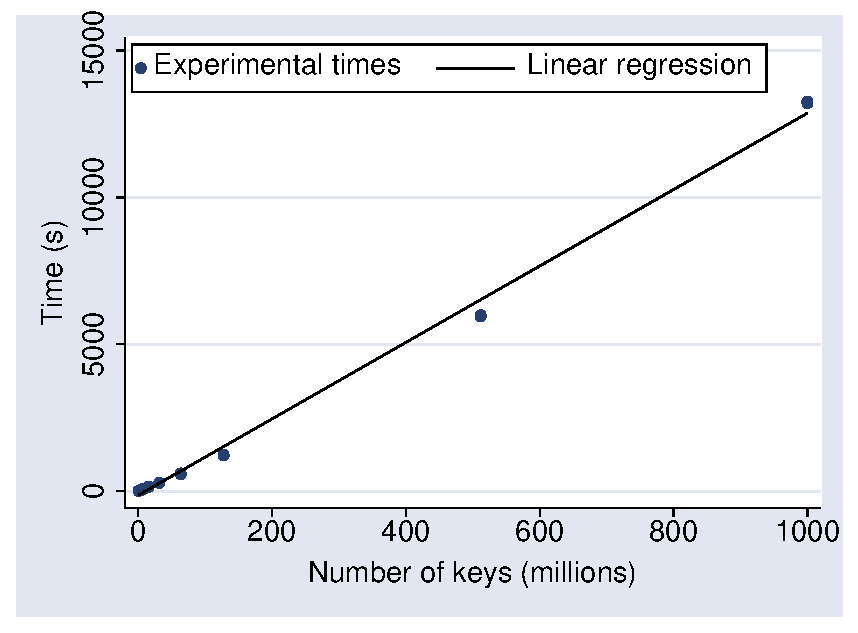
\includegraphics{figs/brz_temporegressao.eps}}
\caption{Time versus number of keys in $S$ for our algorithm. The solid line corresponds to 
a linear regression model.}
\label{fig:brz_temporegressao}
\end{center}
\vspace{-9mm}
\end{figure}

An intriguing observation is that the runtime of the algorithm is almost
deterministic, in spite of the fact that it uses as building block an
algorithm with a considerable fluctuation in its runtime.  A given bucket~$i$,
$0 \leq i < \lceil n/b \rceil$, is a small set of keys (at most 256 keys) and,
as argued in Section~\ref{sec:intern-memory-algor}, the runtime of the
building block algorithm is a random variable~$X_i$ with high fluctuation.
However, the runtime~$Y$ of the searching step of our algorithm is given
by~$Y=\sum_{0\leq i<\lceil n/b\rceil}X_i$.  Under the hypothesis that
the~$X_i$ are independent and bounded, the {\it law of large numbers} (see,
e.g., \cite{j91}) implies that the random variable $Y/\lceil n/b\rceil$
converges to a constant as~$n\to\infty$.  This explains why the runtime of our
algorithm is almost deterministic.


